\section{AL\_\-TC  Class Reference}
\label{classAL__TC}\index{AL_TC@{AL\_\-TC}}
{\tt \#include $<$dil2al.hh$>$}

Inheritance diagram for AL\_\-TC::\begin{figure}[H]
\begin{center}
\leavevmode
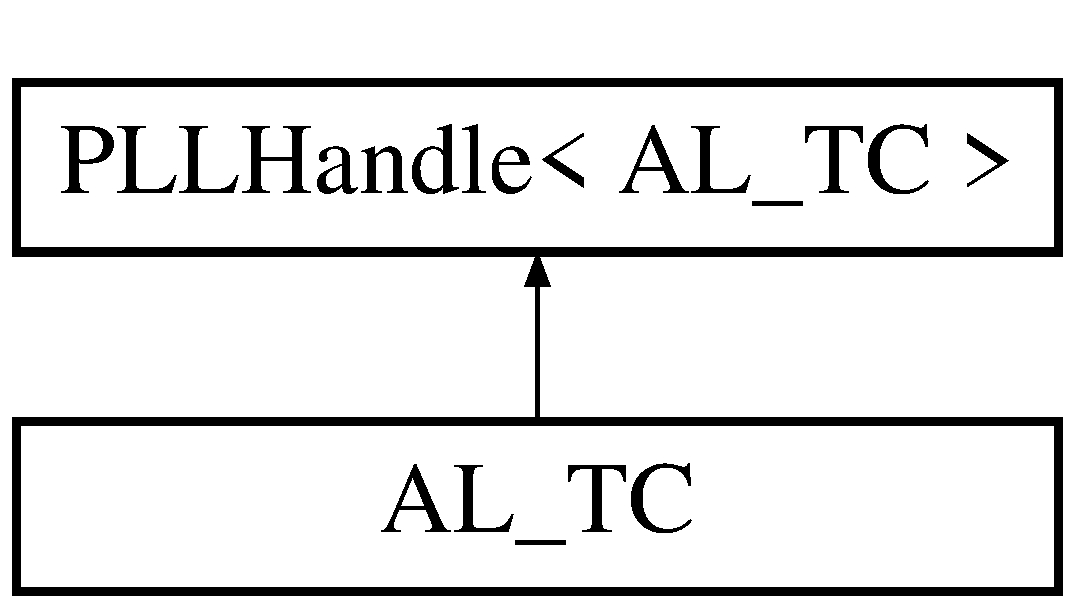
\includegraphics[height=2cm]{classAL__TC}
\end{center}
\end{figure}
\subsection*{Public Methods}
\begin{CompactItemize}
\item 
{\bf AL\_\-TC} ()
\item 
{\bf AL\_\-TC} (long itc, long i\_\-limit)
\item 
{\bf $\sim$AL\_\-TC} ()
\item 
AL\_\-TC $\ast$ {\bf next\_\-avail\_\-el} ()
\item 
AL\_\-TC $\ast$ {\bf avail\_\-el} (unsigned int n)
\item 
void {\bf set\_\-val} (float v)
\item 
{\bf DIL\_\-entry} $\ast$ {\bf Get\_\-DE} ()
\item 
{\bf operator DIL\_\-entry $\ast$} ()
\item 
long {\bf available\_\-before} (unsigned int n)
\item 
float {\bf allocate\_\-with\_\-value} (float uval, {\bf DIL\_\-entry} $\ast$d)
\item 
{\bf DIL\_\-entry} $\ast$ {\bf Set\_\-DE} ({\bf DIL\_\-entry} $\ast$d)
\item 
AL\_\-TC $\ast$ {\bf allocate} ({\bf DIL\_\-entry} $\ast$d)
\end{CompactItemize}
\subsection*{Protected Attributes}
\begin{CompactItemize}
\item 
{\bf DIL\_\-entry} $\ast$ {\bf de}
\item 
float {\bf val}
\end{CompactItemize}


\subsection{Constructor \& Destructor Documentation}
\index{AL_TC@{AL\_\-TC}!AL_TC@{AL\_\-TC}}
\index{AL_TC@{AL\_\-TC}!AL_TC@{AL\_\-TC}}
\subsubsection{\setlength{\rightskip}{0pt plus 5cm}AL\_\-TC::AL\_\-TC ()\hspace{0.3cm}{\tt  [inline]}}\label{classAL__TC_a0}




Definition at line 811 of file dil2al.hh.

References val.



\footnotesize\begin{verbatim}811 : de(NULL), val(0.0) {}
\end{verbatim}\normalsize 
\index{AL_TC@{AL\_\-TC}!AL_TC@{AL\_\-TC}}
\index{AL_TC@{AL\_\-TC}!AL_TC@{AL\_\-TC}}
\subsubsection{\setlength{\rightskip}{0pt plus 5cm}AL\_\-TC::AL\_\-TC (long {\em itc}, long {\em i\_\-limit})}\label{classAL__TC_a1}




Definition at line 324 of file alcomp.cc.

References linear\_\-distribution(), and val.



\footnotesize\begin{verbatim}324                                   : de(NULL) {
325 // create TC and set value
326         val = linear_distribution((float) itc, (float) i_limit);
327 }
\end{verbatim}\normalsize 
\index{AL_TC@{AL\_\-TC}!~AL_TC@{$\sim$AL\_\-TC}}
\index{~AL_TC@{$\sim$AL\_\-TC}!AL_TC@{AL\_\-TC}}
\subsubsection{\setlength{\rightskip}{0pt plus 5cm}AL\_\-TC::$\sim$AL\_\-TC ()\hspace{0.3cm}{\tt  [inline]}}\label{classAL__TC_a2}




Definition at line 814 of file dil2al.hh.



\footnotesize\begin{verbatim}814 {} 
\end{verbatim}\normalsize 


\subsection{Member Function Documentation}
\index{AL_TC@{AL\_\-TC}!allocate@{allocate}}
\index{allocate@{allocate}!AL_TC@{AL\_\-TC}}
\subsubsection{\setlength{\rightskip}{0pt plus 5cm}AL\_\-TC $\ast$ AL\_\-TC::allocate ({\bf DIL\_\-entry} $\ast$ {\em d})}\label{classAL__TC_a11}




Definition at line 379 of file alcomp.cc.

References de, PLLHandle$<$ AL\_\-TC $>$::Next(), and val.

Referenced by AL\_\-Day::allocate().



\footnotesize\begin{verbatim}379                                      {
380 // allocates d to the first available task chunk
381 // returns the allocated task chunk
382         if (de) {
383                 if (Next()) return Next()->allocate(d);
384                 return NULL;
385         }
386         de = d;
387         val = 0.0;
388         return this;
389 }
\end{verbatim}\normalsize 
\index{AL_TC@{AL\_\-TC}!allocate_with_value@{allocate\_\-with\_\-value}}
\index{allocate_with_value@{allocate\_\-with\_\-value}!AL_TC@{AL\_\-TC}}
\subsubsection{\setlength{\rightskip}{0pt plus 5cm}float AL\_\-TC::allocate\_\-with\_\-value (float {\em uval}, {\bf DIL\_\-entry} $\ast$ {\em d})}\label{classAL__TC_a9}




Definition at line 357 of file alcomp.cc.

References de, EOUT, PLLHandle$<$ AL\_\-TC $>$::Next(), and val.

Referenced by AL\_\-Day::allocate\_\-with\_\-value().



\footnotesize\begin{verbatim}357                                                           {
358 // allocate a DIL entry to a task chunk according to
359 // a random value
360 // returns the value of the allocated task chunk
361 // creates TCs if necessary
362         const char _err_msg[] = "dil2al: Available TC values do not add up to day value in AL_TC::allocate_with_value(), continuing\n";
363         if (de) {
364                 if (Next()) return Next()->allocate_with_value(uval,d);
365                 EOUT << _err_msg;
366                 return 0.0;
367         }
368         if (val<uval) {
369                 if (Next()) return Next()->allocate_with_value(uval-val,d);
370                 EOUT << _err_msg;
371                 return 0.0;
372         }
373         de = d;
374         uval = val;
375         val = 0.0;
376         return uval;
377 }
\end{verbatim}\normalsize 
\index{AL_TC@{AL\_\-TC}!avail_el@{avail\_\-el}}
\index{avail_el@{avail\_\-el}!AL_TC@{AL\_\-TC}}
\subsubsection{\setlength{\rightskip}{0pt plus 5cm}AL\_\-TC $\ast$ AL\_\-TC::avail\_\-el (unsigned int {\em n})}\label{classAL__TC_a4}




Definition at line 335 of file alcomp.cc.

References PLL\_\-LOOP\_\-FORWARD.

Referenced by AL\_\-Day::Get\_\-Avail\_\-TC(), and AL\_\-Day::set\_\-TC\_\-values().



\footnotesize\begin{verbatim}335                                       {
336 // returns the nth available task chunk
337         PLL_LOOP_FORWARD(AL_TC,this,1) if (!e->Get_DE()) {
338                 if (n==0) return e;
339                 n--;
340         }
341         return NULL;
342 }
\end{verbatim}\normalsize 
\index{AL_TC@{AL\_\-TC}!available_before@{available\_\-before}}
\index{available_before@{available\_\-before}!AL_TC@{AL\_\-TC}}
\subsubsection{\setlength{\rightskip}{0pt plus 5cm}long AL\_\-TC::available\_\-before (unsigned int {\em n})}\label{classAL__TC_a8}




Definition at line 344 of file alcomp.cc.

References PLL\_\-LOOP\_\-FORWARD.

Referenced by AL\_\-Day::available\_\-before().



\footnotesize\begin{verbatim}344                                            {
345 // returns the number of task chunks available before the
346 // nth task chunk (i.e. does not include the nth task chunk)
347 // This is used by AL_Day::available_before().
348         long avail = 0;
349         PLL_LOOP_FORWARD(AL_TC,this,1) {
350                 if (n==0) return avail;
351                 if (!e->Get_DE()) avail++;
352                 n--;
353         }
354         return avail;
355 }
\end{verbatim}\normalsize 
\index{AL_TC@{AL\_\-TC}!Get_DE@{Get\_\-DE}}
\index{Get_DE@{Get\_\-DE}!AL_TC@{AL\_\-TC}}
\subsubsection{\setlength{\rightskip}{0pt plus 5cm}{\bf DIL\_\-entry}$\ast$ AL\_\-TC::Get\_\-DE ()\hspace{0.3cm}{\tt  [inline]}}\label{classAL__TC_a6}




Definition at line 819 of file dil2al.hh.

Referenced by generate\_\-AL(), Active\_\-List::generate\_\-focused\_\-AL(), Active\_\-List::generate\_\-wide\_\-AL(), operator DIL\_\-entry $\ast$(), and AL\_\-Day::remove\_\-unused\_\-TCs().



\footnotesize\begin{verbatim}819 { return de; }
\end{verbatim}\normalsize 
\index{AL_TC@{AL\_\-TC}!next_avail_el@{next\_\-avail\_\-el}}
\index{next_avail_el@{next\_\-avail\_\-el}!AL_TC@{AL\_\-TC}}
\subsubsection{\setlength{\rightskip}{0pt plus 5cm}AL\_\-TC $\ast$ AL\_\-TC::next\_\-avail\_\-el ()}\label{classAL__TC_a3}




Definition at line 329 of file alcomp.cc.

References PLL\_\-LOOP\_\-FORWARD.



\footnotesize\begin{verbatim}329                              {
330 // returns the next available task chunk
331         PLL_LOOP_FORWARD(AL_TC,this,1) if (!e->Get_DE()) return e;
332         return NULL;
333 }
\end{verbatim}\normalsize 
\index{AL_TC@{AL\_\-TC}!operator DIL_entry *@{operator DIL\_\-entry $\ast$}}
\index{operator DIL_entry *@{operator DIL\_\-entry $\ast$}!AL_TC@{AL\_\-TC}}
\subsubsection{\setlength{\rightskip}{0pt plus 5cm}AL\_\-TC::operator {\bf DIL\_\-entry} $\ast$ ()\hspace{0.3cm}{\tt  [inline]}}\label{classAL__TC_a7}




Definition at line 820 of file dil2al.hh.

References Get\_\-DE().



\footnotesize\begin{verbatim}820 { return Get_DE(); }
\end{verbatim}\normalsize 
\index{AL_TC@{AL\_\-TC}!Set_DE@{Set\_\-DE}}
\index{Set_DE@{Set\_\-DE}!AL_TC@{AL\_\-TC}}
\subsubsection{\setlength{\rightskip}{0pt plus 5cm}{\bf DIL\_\-entry}$\ast$ AL\_\-TC::Set\_\-DE ({\bf DIL\_\-entry} $\ast$ {\em d})\hspace{0.3cm}{\tt  [inline]}}\label{classAL__TC_a10}




Definition at line 826 of file dil2al.hh.

Referenced by AL\_\-Day::add\_\-TCs().



\footnotesize\begin{verbatim}826 { DIL_entry * dprev = de; de = d; return dprev; }
\end{verbatim}\normalsize 
\index{AL_TC@{AL\_\-TC}!set_val@{set\_\-val}}
\index{set_val@{set\_\-val}!AL_TC@{AL\_\-TC}}
\subsubsection{\setlength{\rightskip}{0pt plus 5cm}void AL\_\-TC::set\_\-val (float {\em v})\hspace{0.3cm}{\tt  [inline]}}\label{classAL__TC_a5}




Definition at line 818 of file dil2al.hh.

References val.

Referenced by AL\_\-Day::set\_\-TC\_\-values().



\footnotesize\begin{verbatim}818 { val = v; }
\end{verbatim}\normalsize 


\subsection{Member Data Documentation}
\index{AL_TC@{AL\_\-TC}!de@{de}}
\index{de@{de}!AL_TC@{AL\_\-TC}}
\subsubsection{\setlength{\rightskip}{0pt plus 5cm}{\bf DIL\_\-entry}$\ast$ AL\_\-TC::de\hspace{0.3cm}{\tt  [protected]}}\label{classAL__TC_n0}




Definition at line 807 of file dil2al.hh.

Referenced by allocate(), and allocate\_\-with\_\-value().\index{AL_TC@{AL\_\-TC}!val@{val}}
\index{val@{val}!AL_TC@{AL\_\-TC}}
\subsubsection{\setlength{\rightskip}{0pt plus 5cm}float AL\_\-TC::val\hspace{0.3cm}{\tt  [protected]}}\label{classAL__TC_n1}




Definition at line 808 of file dil2al.hh.

Referenced by AL\_\-TC(), allocate(), allocate\_\-with\_\-value(), and set\_\-val().

The documentation for this class was generated from the following files:\begin{CompactItemize}
\item 
{\bf dil2al.hh}\item 
{\bf alcomp.cc}\end{CompactItemize}
